\section{Introduction}\label{sec:intro}

The latent width of a variational autoencoder (VAE)~\cite{kingma2014vae}
controls the capacity available to its representation. Choosing that width
by validation over a candidate grid is straightforward, but requires
training several models. Alternatives include intrinsic-dimension (ID)
estimation~\cite{facco2017twonn,levina2005mle}, comparisons between sampled
and mean latent representations~\cite{bonheme2022fondue}, activity
diagnostics~\cite{burda2016iwae,bonheme2023active}, and pruning through
reconstruction constraints or relevance priors~\cite{deboom2020geco,saha2025ardvae}.
These signals answer different questions: geometric dimension, coordinate
use, reconstruction quality and network width need not coincide.

This study asks whether ID guidance reduces the recorded training cost of
finding a small VAE that meets a stated reconstruction target, whether AU
diagnostics provide information beyond other recorded quantities, and how
selection changes with regularisation and readout settings. We compare
selection rules using the same candidate-model families, data splits and
quality yardstick. For pruning approaches, we explicitly evaluate
\emph{dimension transfer}: a returned count is mapped to a grid width and
used to select an ordinary VAE. This comparison does not measure the
performance of the original pruned or hierarchical-prior model.

The contribution is a conditional empirical comparison and an audit of
what its measurements support. Four image datasets and five
candidate-training seeds are represented. The regularisation analysis
uses five weights, but its intervention differs for the pruning
adaptations, as specified below. We provide numerical quality targets,
test results, learning curves, paired readout analyses, and the executed
ID-guided procedure. We distinguish algorithmic termination, fallback,
quality attainment and compression, and separate measured training time
from unmeasured overhead.

At the primary MNIST setting, ID guidance and ascending search return the
same six-dimensional model, with recorded training accounts of 715 and
182~s, respectively. This supports a narrow conclusion about that
implementation and target. The other results describe dependence on
representations, training settings and diagnostic thresholds; they do not
establish a universal ordering of selection methods. Experimental details
are given in Sections~\ref{sec:framework}--\ref{sec:setup}, results in
Section~\ref{sec:results}, and limitations in Section~\ref{sec:discussion}.

\section{Related Work}\label{sec:related}

\subsection{Dimension, Reconstruction and Latent Activity}
PCA~\cite{tippingbishop1999ppca}, Isomap~\cite{tenenbaum2000isomap} and
locally linear embedding~\cite{roweis2000lle} construct low-dimensional
representations. ID estimators instead quantify local dimension from
sample geometry. We use TwoNN and an MLE cross-check; other approaches
include DANCo, expected simplex skewness and geodesic entropic
graphs~\cite{ceruti2014danco,johnsson2015ess,costa2004geodesic}.
Estimator limitations and dependence on the sampled distribution motivate
cross-checks~\cite{camastra2016intrinsic,allegra2020data}.
Graph-based methods are outside this experiment's scope; we do not infer
that they would resolve or reproduce the observed disagreements.
Lower ID in learned representations has also been observed in deep
networks~\cite{ansuini2019intrinsic,pope2021intrinsic}.

FONDUE~\cite{bonheme2022fondue} searches for the capacity preceding a
separation between ID estimates of sampled and posterior-mean
representations. Its appendix gives FONDUE-VAR, which chooses a count from
latent-variable types. AU and variable types share an interest in unused
coordinates but are different statistics: AU thresholds the across-data
variance of posterior means, whereas the type classifier uses moments of
posterior variances~\cite{bonheme2023active}. Agreement of their final
counts is not equivalence of their stability or information content.

GECO with $L_0$ regularisation optimises a gated VAE under a reconstruction
constraint, with KL and gate-count terms~\cite{deboom2020geco,rezende2018geco}.
The source uses ARM; our adaptation uses hard-concrete
gates~\cite{louizos2018l0}. Neither the nonconvex optimisation nor our
implementation guarantees a global minimum capacity. Our validation
anchor plus tolerance is a particular way of setting an external quality
yardstick, not an identical implementation of the source's constraint.

ARD-VAE uses a hierarchical relevance prior~\cite{saha2025ardvae}.
The source tunes a regularisation weight, uses a Gaussian approximation
for its closed-form KL, and selects axes explaining 99\% of a
Jacobian-weighted variance score. It is therefore not threshold-free.
The local adaptation has additional differences, including a finite-step
decoder score and a fixed selection-stage weight; these are detailed in
Appendix~\ref{app:adaptations}.

\subsection{Relation to the Conference Paper and Earlier Manuscript}
Our NOLTA2025 contribution~\cite{obata2025manifold} concerned the relation
between input ID and latent-space capacity. The available conference
manuscript describes class-specific MNIST experiments with four fully
connected and two convolutional architectures and four seeds. CNNs and
multiple seeds are consequently not new features of this revision.
The conference manuscript available for comparison has a working title
different from the published title; the reference uses the title and
pages listed by the authors' institutional publication record.
Table~\ref{tab:history} distinguishes this earlier scope from the present
comparison. MAKE47 denotes the earlier journal submission, not a separate
publication.

\begin{table}[H]
\caption{Scope of the conference study, earlier journal submission and present revision.}
\label{tab:history}\small
\begin{tabularx}{\textwidth}{lXXX}\toprule
Item & NOLTA2025 & MAKE47 & Present revision \\\midrule
Question & Input and latent ID versus capacity & ID-guided choice with AU verification & Selection quality, cost and diagnostic limitations \\
Models & Four FC and two CNN structures; MNIST classes; four seeds & FC/CNN and synthetic/image extensions & Fixed candidate families on four image datasets; five candidate seeds \\
Comparators & Architecture and capacity comparisons & Capacity sweeps and diagnostic checks & FONDUE variants, pruning adaptations, grid criteria and ascending search \\
Readouts & ID estimates & AU-based operational checks & Same-checkpoint type/AU trajectories and paired predictive analysis \\
Evidence & Conference settings & Earlier loss convention & Corrected-loss records; explicit targets, final test metrics and accounting limits \\
\bottomrule\end{tabularx}
\end{table}

\section{Evaluation Framework}\label{sec:framework}

\subsection{Models and Quality Target}\label{sec:quality}
We distinguish the \emph{ID-reference AE}, which supplies a representation
for estimation, the \emph{quality anchor}, an ordinary VAE at the largest
candidate width, and the \emph{selected model}, the ordinary VAE evaluated
after dimension selection. Write $\mathcal M$ for the candidate grid,
$s$ for a training seed, and $D_s(m,\beta)$ for validation per-pixel MSE
of the deterministic reconstruction $g(\mu(x))$. The implemented target is
\begin{align}
 m_a&=\max\mathcal M, &
 T_{D,s}(\beta)&=D_s(m_a,\beta)
 +\max\{0.10D_s(m_a,\beta),\,0.001\operatorname{Var}(X_{\rm val})\}.
 \label{eq:target}
\end{align}
The variance is computed over all validation-array entries. The relative
term dominates in every recorded image condition, giving
$T_{D,s}=1.10D_s(m_a,\beta)$. The configuration originally also specified a
three-seed-SD term, but the executed target function was supplied one
anchor at a time and omitted that term. We report the implemented rule;
we do not retrospectively describe it as a pooled-seed target.
Appendix~\ref{app:targets} lists every dataset--$\beta$ anchor and target.

For a fixed seed and $\beta$, the target is held constant during search.
It is recomputed from a different anchor when $\beta$ changes. A
$\beta$-sweep therefore changes both the learned representation and the
quality yardstick. It is not a fixed-quality intervention. A method that
returns a valid width need not meet this external target; quality
attainment is evaluated separately for every final model.

\subsection{Cost Accounting and Shared Candidates}\label{sec:cost}
Candidates with the same dataset, architecture, likelihood, width, seed,
epoch budget, stopping option and $\beta$ are shared through a cache.
Each selection rule is charged the recorded training duration of every
distinct candidate it requests. Reusing a candidate within the rule costs
no additional training time. Consequently, identical selected candidates
have identical metrics across methods. They are paired observations, not
independently retrained method-specific models. A selected candidate
already trained during search is reused; a short-search candidate receives
the ordinary final training schedule.

The original ledgers did not charge the quality anchor to every method.
For this revision, its recorded duration is added wherever absent; if it
is also the final ordinary VAE, it is counted once. The resulting
$C_{\rm train}$ includes candidate training, ID-reference AE training,
the anchor, and separately recorded probe time where used for selection.
Training timers include epoch-wise validation, but omit several
post-training evaluations and ID computations. The pruning timers have
slightly different boundaries, including their final readout. Thus
$C_{\rm train}$ is an attributed recorded-time account, not an end-to-end
wall-clock measurement. Exact overhead cannot be recovered from these
logs. FONDUE epoch-calibration time is reported separately because it is
performed once per dataset--$\beta$ condition. No complete wall-clock
speedup is claimed.

\subsection{Outputs and Termination}\label{sec:outcomes}
Each trial records a raw returned dimension, the width of the evaluated
model, the ID reliability decision where applicable, fallback use, the
logged termination state, the budget flag, quality attainment, and whether
the final width is smaller than the anchor. These events can overlap.
In particular, fallback can produce a compact model that meets the target.
The label \texttt{SUCCESS} in an older log indicates ordinary termination;
it is not itself evidence of target attainment.

A budget-exceeded trial contributes its consumed time and, if it has a
returned model, that model's dimension and metrics. A raw dimension below
one is reported as degenerate; its time and failure count remain, while
MSE is missing because no final model exists. The original implementation
checks budgets after completed calls and can still obtain a final model.
The reported limits are therefore soft accounting limits, not hard
interruptions. Outcome tables preserve these distinctions.

\subsection{Executed ID-Guided Procedure}\label{sec:algorithm}
Algorithm~\ref{alg:id} describes the executed selection rather than a
hypothetical improved variant. The reference bank uses three widths and
three fixed reference seeds, shared across the five candidate seeds.
Let $\bar d_r$ be the mean TwoNN estimate at reference width $r$,
$\hat d=\operatorname{mean}_r\bar d_r$, and $\bar d_{\rm MLE}$ the mean
MLE estimate over that same bank. The checks are
\begin{equation}
 R=\frac{\max_r\bar d_r-\min_r\bar d_r}{\operatorname{median}_r\bar d_r}
 \le0.15,\qquad
 A=\frac{|\hat d-\bar d_{\rm MLE}|}{\hat d}\le0.25.
 \label{eq:checks}
\end{equation}
The implemented initial window includes every grid point at or below the
first grid point greater than or equal to $2\hat d$, not only points
between $\hat d$ and $2\hat d$.

\noindent\begin{minipage}{\linewidth}
\begin{Algorithm}[Executed ID-guided selection and external evaluation]
\label{alg:id}\normalfont\small\leavevmode\par\noindent
\textbf{Input:} splits, $\mathcal M$, seed $s$, $\beta$, 10\% target margin,
floor coefficient 0.001, input TwoNN $d_0$, reference seeds
$\{42,123,777\}$, thresholds $(0.15,0.25)$, and budgets in Table~\ref{tab:data}.
\begin{enumerate}
\item Obtain the quality anchor and fix $T_{D,s}$ from
Equation~\eqref{eq:target}. In a fallback run this is an external audit
step, not a constraint used by the coarse selector; its training is charged.
\item For $k\in\{4,8,16\}$ set $r_k=\operatorname{round}(kd_0)$
(nearest integer; ties to even, no grid snapping). Train an FC-AE at each
width for each reference seed, and compute TwoNN and MLE on the fixed
10,000 training examples. Compute $R$, $A$ and $\hat d$.
\item If either check fails, flag ID-unreliable and evaluate the coarse
subset. Its zero-based indices are the unique values of
$\operatorname{round}(\operatorname{geomspace}(1,|\mathcal M|,4))-1$.
Return its minimum-validation-MSE candidate and continue to step 6.
\item Otherwise set $m_0=\min\{m\in\mathcal M:m\ge2\hat d\}$,
or $m_a$ if the set is empty. Initialise the evaluated set with the
anchor. Evaluate all remaining $m\le m_0$ in ascending order, stopping
after a completed call that exceeds the budget.
\item Return the smallest target-satisfying width in the evaluated set.
If it is the anchor, record no compact alternative. The anchor is always
acceptable; the code's planned expansion conditional on \emph{no}
acceptable evaluated candidate is consequently never reached.
\item Obtain or reuse the ordinary VAE at the returned width. For
$m<1$ return a degenerate output with no model. Retain budget flags even
when a model is returned. Record AU as a diagnostic without changing $m$.
\item Return raw and final widths, model metrics, ID diagnostics,
fallback and budget flags, quality/compression indicators and the time account.
\end{enumerate}
\end{Algorithm}
\end{minipage}

The unreachable expansion branch limits the implemented ID-guided
selector. It is disclosed rather than silently repaired while retaining
old outcomes. The MNIST primary selection occurs within the initial
window, so the reported comparison there does not require expansion.
The earlier V1/V2 activity checks are not selection branches in this
revision. Ascending search uses the same anchor and target, scans upwards
to the first acceptable candidate, and requires no ID-reference AEs.

\section{Theoretical Background}\label{sec:theory}
For an ideal smooth $d$-manifold, Whitney's embedding theorem gives an
embedding into $\mathbb R^{2d}$~\cite{whitney1944}. Exact continuous
reconstruction through an injective encoder entails an embedding, but
neither a noisy finite-sample ID estimate nor an approximate neural
reconstruction satisfies these assumptions automatically. The multiplier
two is therefore a heuristic under evaluation, not a quality guarantee or
a lower bound inferred from measured ID.

In linear Gaussian latent-variable models, informative directions depend
on the covariance spectrum and noise scale; analyses of linear VAEs and
posterior collapse make this relation explicit~\cite{tippingbishop1999ppca,lucas2019elbo}.
VAE alignment with principal directions has also been
studied~\cite{rolinek2019pca}. These results motivate measuring how
regularisation affects coordinate use. They do not equate AU with
intrinsic or minimum embedding dimension in a nonlinear VAE. AU also
depends on the latent coordinates and the threshold used to count them.

\section{Experimental Setup}\label{sec:setup}

\subsection{Data, Architecture and Optimisation}
Table~\ref{tab:data} gives the actual image-data settings.
MNIST~\cite{lecun1998}, Fashion-MNIST~\cite{xiao2017fashion} and
CIFAR-10~\cite{krizhevsky2009learning} use random subsets of the official
training and test pools. A permutation with seed 20260912 selects 20,000
training-pool examples; another with seed 20260913 divides them 90:10.
The 3000 test examples use seed 20260914. For
dSprites~\cite{matthey2017dsprites}, which has no official train/test
split, the first 20,000 and next 3000 entries of one permutation of
737,280 images are disjoint pools; the 20,000 are divided 90:10 and each
index list is sorted before loading. Images are scaled to $[0,1]$, with
no augmentation. Training seeds are $42,123,777,2024,31337$; the split
does not vary with these seeds.

\begin{table}[H]
\caption{Image-data settings used for candidate VAEs. All datasets use
18,000 training, 2000 validation and 3000 test examples. G: Gaussian;
B: Bernoulli. Budgets are recorded-time limits with a common limit of
12 candidate-training calls; ID AEs are additional.}
\label{tab:data}\small
\begin{tabularx}{\textwidth}{lccXr}\toprule
Dataset & Input & Likelihood & Candidate widths & Budget (s) \\\midrule
MNIST & $1\times28\times28$ & G & 2, 4, 6, 8, 10, 12, 16, 20, 24, 32, 48, 64 & 1470 \\
Fashion-MNIST & $1\times28\times28$ & G & Same as MNIST & 1470 \\
dSprites & $1\times64\times64$ & B & Same as MNIST & 5163 \\
CIFAR-10 & $3\times32\times32$ & G & 8, 16, 24, 32, 48, 64, 96, 128, 192, 256 & 2924 \\
\bottomrule\end{tabularx}
\end{table}

For MNIST and Fashion-MNIST, the encoder has dense widths 512 and 256,
ReLU activations, and separate linear mean/log-variance heads; the decoder
has widths 256 and 512 with a linear output. The CIFAR-10 encoder has
channels 32, 64 and 128; dSprites adds 256. Convolutions use kernel 4,
stride 2, padding 1 and ReLU, leaving $4\times4$ feature maps, followed
by linear posterior heads. A linear/ReLU projection and reversed
transposed convolutions form the decoder, ending in a sigmoid. The
ID-reference AE flattens the input and uses dense widths 512--256--$r$
and the reverse decoder, with a linear output; it is separate from the
candidate CNNs.

Ordinary candidates use Adam, learning rate $10^{-3}$, default moments
$(0.9,0.999)$, $\epsilon=10^{-8}$, no weight decay, batch size 128 and
up to 300 epochs. The last batch has 80 examples (141 updates per epoch).
ID AEs use the same optimiser and batch size for 100 epochs.
Early stopping uses patience 30. A recorded plateau flag requires
$(\max h-\min h)/|\operatorname{mean}h|<0.01$ over the last 50
validation-monitor values. It is not an additional stopping rule.
Representative trajectory runs always complete 300 epochs.

The candidate training loss is
\begin{equation}
 \mathcal L_\beta=\frac1B\sum_{i=1}^B
 \left[\ell(x_i,g(z_i))+\beta\sum_{j=1}^{m}
 \frac{\mu_{ij}^2+\exp(v_{ij})-1-v_{ij}}{2}\right],
 \qquad z_i\sim q_\phi(z\mid x_i),
 \label{eq:loss}
\end{equation}
where $v$ is log variance. Gaussian reconstruction uses a sum of squared
errors, equivalent to fixed observation variance $1/2$ up to an additive
constant; dSprites uses summed binary cross-entropy. The primary weight
is one; the ladder is $\{0.25,0.5,1,2,4\}$, constant during each run.
No cyclical annealing schedule~\cite{fu2019cyclical} is used.
Equal numerical $\beta$ across likelihoods does not imply equal
regularisation strength.

The stored validation monitor named ``ELBO'' is
$h=-[\ell(x,g(\mu(x)))+\mathrm{KL}]$, averaged over examples. It uses
posterior-mean reconstruction, not an expectation over posterior samples,
and is therefore an \emph{ELBO proxy}, not an unbiased ELBO estimate or a
certified bound. It also uses unit KL weight for checkpoint selection
even when training uses another $\beta$. We retain these checkpoints and
label the monitor accurately. No test metric enters the selection code.
However, the candidate cache evaluates test metrics for every trained
candidate, before method selection; the claim that only one final test
evaluation was executed would be incorrect. Tables report test metrics
only for the validation-selected models. This is a code-level separation
of selection and evaluation, not a prospectively sealed test workflow.

\subsection{Methods and Readouts}\label{sec:methods}
Grid search selects by validation MSE, the ELBO proxy, or linear-probe
validation accuracy. Probes use posterior means, multinomial logistic
regression, up to 2000 iterations, and
$C\in\{0.01,0.1,1,10\}$ chosen by validation. Labels are digit/apparel/
CIFAR classes and the three dSprites shapes. Both capacity and probe
regularisation use validation labels in the probe selector. Coarse search
uses Algorithm~\ref{alg:id}'s subset; the fixed baseline uses width 32.

FONDUE is a local PyTorch implementation using TwoNN and a fixed
ID-gap threshold $0.2d_0$. It searches integer widths, which can lie
outside the ordinary candidate grid. Its selected width is trained
exactly. At $\beta=1$, short training uses one epoch for MNIST and
dSprites and two for Fashion-MNIST and CIFAR-10. dSprites follows the
source's epoch choice; elsewhere a seed-42 calibration increases epochs
until two consecutive predictions agree, stopping at five. Other
$\beta$-specific choices are in Appendix~\ref{app:coverage}.
FONDUE+$Q$ maps the returned width upwards onto the grid, obtains the
anchor, and extends upwards until quality is met or its budget flag is
set. This adds an external reconstruction rule to FONDUE.

FONDUE-VAR starts at $\operatorname{round}(2d_0)$ and doubles width until
the declared type condition is met. With mixed variables kept it returns
active plus mixed once a passive variable appears; otherwise it returns
the active count once a mixed or passive variable appears. We implement
the description-based classifier: posterior variance is exponentiated
\emph{once} from log variance. A coordinate is passive if its across-data
variance is below 0.1 and its mean is in $[0.9,1.1]$, active if that
variance is below 0.1 and its mean is at most 0.1, and mixed otherwise.
The audited public-code version is identified in
Appendix~\ref{app:adaptations}; this is not claimed to reproduce every
path of that code or its published experimental settings.

AU is independently defined by
\begin{equation}
 \mathrm{AU}_\delta=\sum_{j=1}^{m}
 \mathbf1\{\operatorname{Var}_{x\in X_{\rm est}}\mu_j(x)>\delta\},
 \qquad \delta\in\{10^{-3},10^{-2},10^{-1}\},
 \label{eq:au}
\end{equation}
with primary $\delta=10^{-2}$. ID and activity readouts use the same
10,000 training examples sampled without replacement using seed
20260915. The MLE cross-check uses $k=10$ neighbours. AU is diagnostic,
not an extra selector in the method comparison.

The GECO and ARD adaptations start at the largest grid width and run
300 epochs. Their raw coordinate counts are mapped to the nearest
candidate width, with ties going to the smaller width, for the final
ordinary VAE. Appendix~\ref{app:adaptations} specifies the local
objectives, updates and readout differences. The evaluated MSE thus
belongs to the transferred ordinary VAE, not to the original model.

\subsection{Provenance and Scope of Prior Specification}\label{sec:provenance}
The saved image-experiment provenance is Python 3.12.3, PyTorch
2.7.1+cu118, CUDA 11.8, cuDNN 90100 (9.1.0), NVIDIA driver 570.211.01,
and an NVIDIA GeForce RTX 3070, on Linux 6.8.0-124-generic, x86-64,
glibc 2.39. GPU provenance is recorded for these experiments; CPU
numerical and probe operations accompany GPU training. The earlier
MAKE47 manuscript did state PyTorch 2.0, RTX 3070 and a CPU fallback;
it did not identify the complete CUDA/cuDNN/driver environment.

The configuration file was created on 12 September 2026, with subsequent
changes recorded on 12--13 September. These are internal specification
records, not a public preregistration. Calibration informed some changes,
including the dSprites likelihood. The pruning additions and full ladder
were run during 14--17 September. The paired random-feature comparison
and accounting audit here are retrospective revisions dated 18 September.
MNIST and other previously examined datasets are not described as wholly
unseen scientific conditions. ``Evaluation condition'' in the predictive
analysis means withheld from fitting that predictor.

The logged code token \texttt{8c2c6c28224b3450} hashes only the common
module and configuration, not the entire experimental implementation;
the earlier trajectory records use \texttt{99cb5eb7404ff6e7}.
A new SHA-256 file manifest identifies the inspected snapshot.
Appendix~\ref{app:inventory} maps numerical results to their source files
and describes remaining provenance limitations.

\section{Results}\label{sec:results}

\subsection{Selection Quality and Recorded Cost}
Tables~\ref{tab:main1} and \ref{tab:main2} include all four datasets at
$\beta=1$, with mean and sample SD over five candidate-training seeds.
They report final model widths, validation and test error, quality
attainment and the corrected training-time account. Independent outcome
counts appear in Appendix~\ref{app:outcomes}. These uncertainty summaries
are conditional on one split and, for ID guidance, one shared reference
bank.

@@table:main1@@
@@table:main2@@

On MNIST, ID guidance and ascending search return $m=6$ in all five
trials and share the same final models. Their validation MSE is 0.02244;
all meet the target. The recorded training accounts are 715 and 182~s,
respectively (a ratio of approximately 3.9). The difference mainly
reflects the reference-AE bank and additional candidates
(Table~\ref{tab:cost}); its missing ID-estimation overhead cannot support
a more favourable ID cost. It remains a comparison of the executed
procedures rather than proof that every possible ID-guided search is
slower.

On dSprites, ordinary FONDUE returns approximately four dimensions but
has validation MSE 0.00550, versus 0.00126 for ascending search. The
target column shows whether this faster selection reaches comparable
quality. Normal termination alone must not be read as quality success.
The FONDUE+$Q$ dSprites result includes one budget-exceeded trial with
an existing returned model; it is retained in the means.

The ID check fails on Fashion-MNIST, dSprites and CIFAR-10, so those
rows are coarse-search fallbacks with the reference cost added. They are
not examples of successful ID placement. The high variability on
CIFAR-10 belongs to this fallback. dSprites is a synthetic image dataset;
the only natural colour-image benchmark here is CIFAR-10.

@@table:cost@@

\begin{figure}[!htbp]
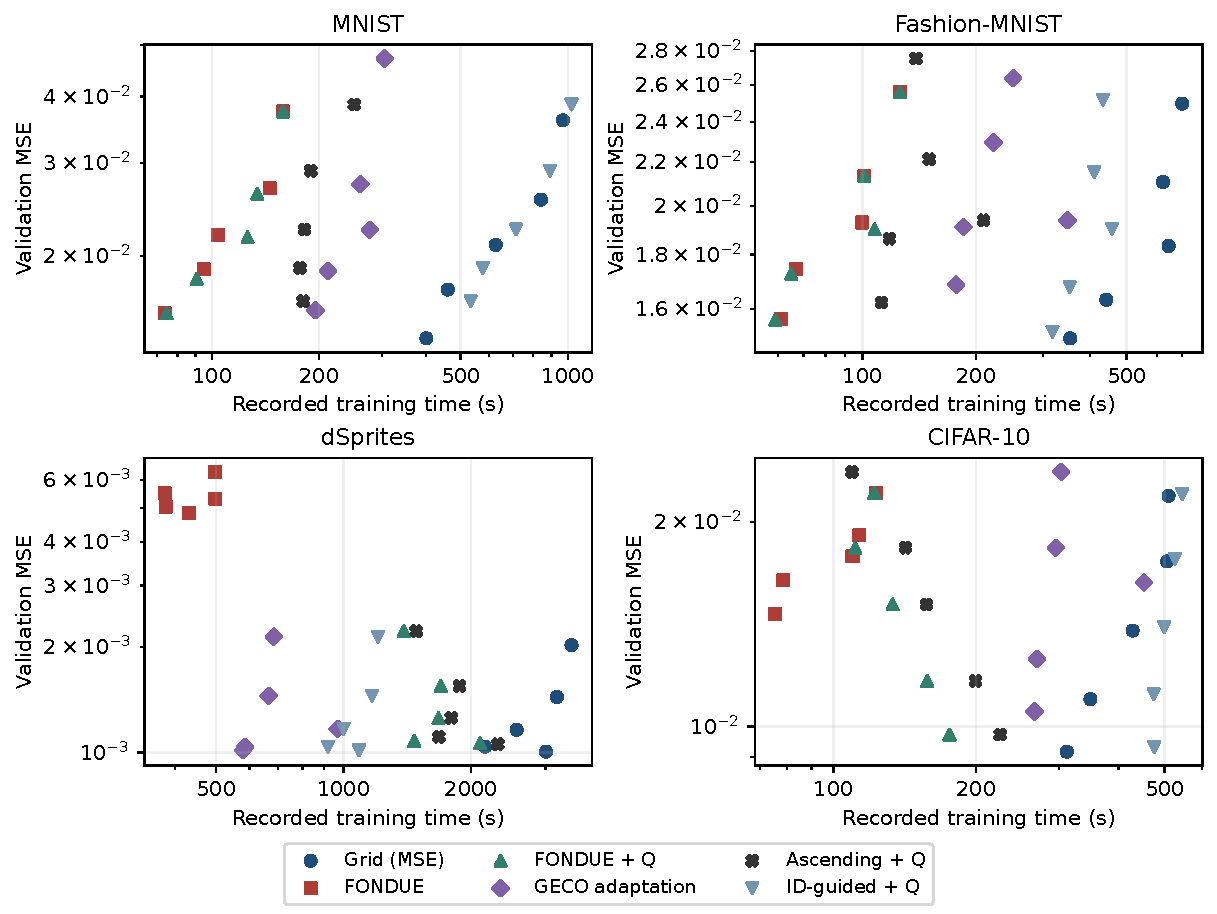
\includegraphics[width=\textwidth]{results/figures/MAKE50/quality_cost.pdf}
\caption{Validation quality versus attributed recorded training time,
five seed means for each of five regularisation settings. Gaussian
likelihood except Bernoulli dSprites. ARD is omitted because its selection
stage did not vary with $\beta$. GECO changes the anchor-derived
constraint. These points do not all meet a common fixed-quality target.}
\label{fig:cost}
\end{figure}

\subsection{Representation and Sample Dependence of ID}
Table~\ref{tab:id} gives the complete reference-bank summary, including
Fashion-MNIST. Only MNIST passes both checks. Because the same bank is
reused, five identical pass/fail decisions do not constitute five
independent replications of ID estimation.

@@table:id@@

Figure~\ref{fig:id} separately shows the sample-size and PCA analyses.
At 1000 examples the two estimators agree within the specified 0.25
relative tolerance on all four raw-input datasets; at 10,000, only MNIST
does. These are raw-input checks, distinct from the AE-latent checks used
by the selector. On dSprites, input TwoNN is 7.70 in this diagnostic,
PCA estimates range from 2.68 to 4.32, and individual AE estimates range
from 2.08 to 4.56. The combined range is about 3.7-fold; the corresponding
MNIST range is about 1.7-fold. These are representation-dependent
estimates, not competing measurements of a known ground truth.

\begin{figure}[!htbp]
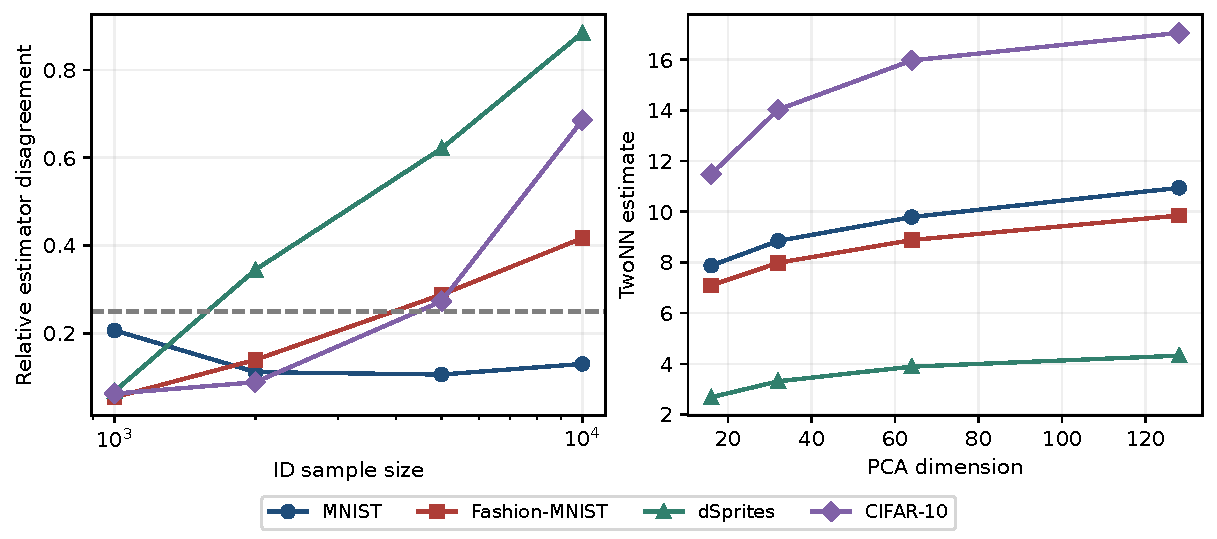
\includegraphics[width=\textwidth]{results/figures/MAKE50/id.pdf}
\caption{Left: $|d_{\rm TwoNN}-d_{\rm MLE}|/d_{\rm TwoNN}$ on raw
inputs as estimation sample size changes; dashed line is 0.25. Right:
TwoNN after PCA preprocessing. PCA rank, sample size and representation
are distinct interventions; AE results are in Table~\ref{tab:id}.}
\label{fig:id}
\end{figure}

\subsection{Dependence on Regularisation and Quality Context}\label{sec:beta}
Define the reported range for method $a$ and dataset $d$ by
\begin{equation}
 S_{a,d}=\max_{\beta\in\mathcal B}\bar m_{a,d}(\beta)
         -\min_{\beta\in\mathcal B}\bar m_{a,d}(\beta),\qquad
 \bar m_{a,d}(\beta)=\frac15\sum_{s=1}^{5}m_{a,d,s}(\beta),
 \quad\mathcal B=\{0.25,0.5,1,2,4\}.
 \label{eq:span}
\end{equation}
This is the range of seed means of raw returned dimensions, not the mean
of within-seed ranges. For the FONDUE-VAR row all five outputs are
defined at each setting, including any raw zero. It is a descriptive
range on the tested ladder, not a new parameter-free robustness index.

@@table:span@@

Ranges differ by method and dataset, with clear ordering reversals.
For example, ID-guided versus GECO-adaptation ranges are 6.0 versus 8.8
on MNIST, but 214.4 versus 34.2 on CIFAR-10. The latter ID-guided value
is inherited from fallback. A fixed dimension has zero range by design;
dSprites ID fallback has zero range because coarse search always returns
64. Neither demonstrates useful selection robustness. We do not average
ranges across differently scaled grids or assert a transferable ranking.

The ARD call contains no selection-stage $\beta$ argument and optimises
reconstruction plus KL with unit weight every time. Its five contextual
runs repeat the same selection settings and seeds. The final ordinary
VAE changes with the contextual $\beta$, but the ARD-selected count does
not. The former zero-range row is therefore excluded from sensitivity
comparison. GECO has a different intervention: its constraint is
$\tau=T_{D,s}(\beta)$, while its KL coefficient remains one. These
distinctions are explicit in Figure~\ref{fig:beta}.

\begin{figure}[!htbp]
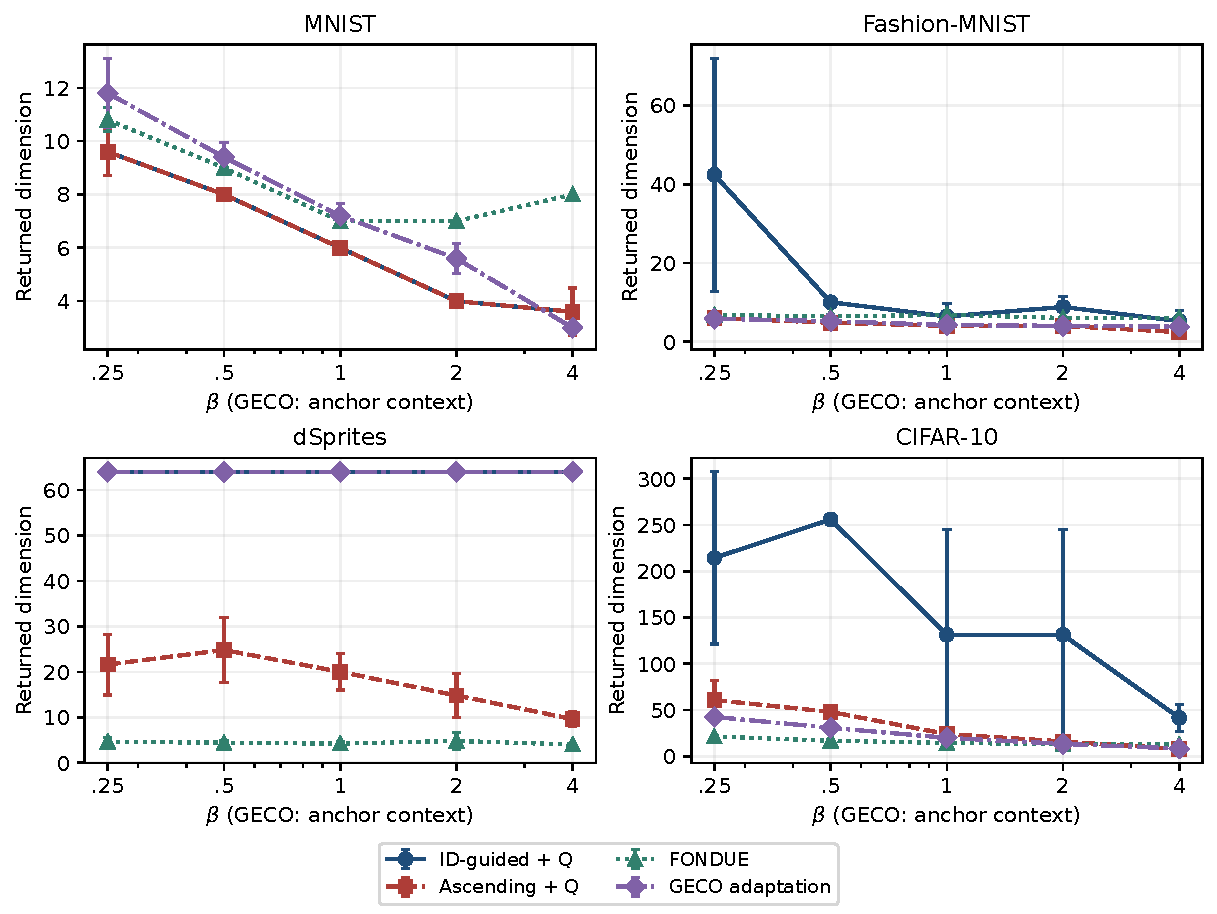
\includegraphics[width=\textwidth]{results/figures/MAKE50/beta.pdf}
\caption{Raw returned dimension across the five contexts, mean $\pm$ SD
over five candidate seeds. Gaussian likelihood except Bernoulli dSprites.
Ordinary VAE selectors change training $\beta$; GECO changes its
anchor-derived constraint. ARD is excluded. ID guidance falls back on
Fashion-MNIST, dSprites and CIFAR-10 throughout the ladder.}
\label{fig:beta}
\end{figure}

An AU-threshold intervention holds the checkpoint fixed and recomputes
Equation~\eqref{eq:au}. A quality-margin intervention instead changes
which cached models satisfy the target. Neither is the same as changing
training $\beta$. We report these readout/quality analyses separately
(Section~\ref{sec:au} and Appendix~\ref{app:sensitivity}). No sensitivity
claim is made for untested FONDUE stopping thresholds or ARD cumulative
relevance fractions.

\subsection{Learning Curves, Test Evaluation and Selection Criteria}
The saved trajectory experiment supplies train/validation curves for
MNIST widths 12, 32 and 64 and dSprites widths 6, 16 and 32, with five
seeds each (Figure~\ref{fig:learning}). Training MSE is evaluated in
deterministic mode on a fixed 2000-example training subset sampled with
seed 20260919. Both train and validation improve, but validation error
remains higher. None of these 30 runs passes the stringent final
50-epoch plateau check; completing 300 epochs is not proof of convergence.
These curves cover representative settings, not all four datasets.

\begin{figure}[!htbp]
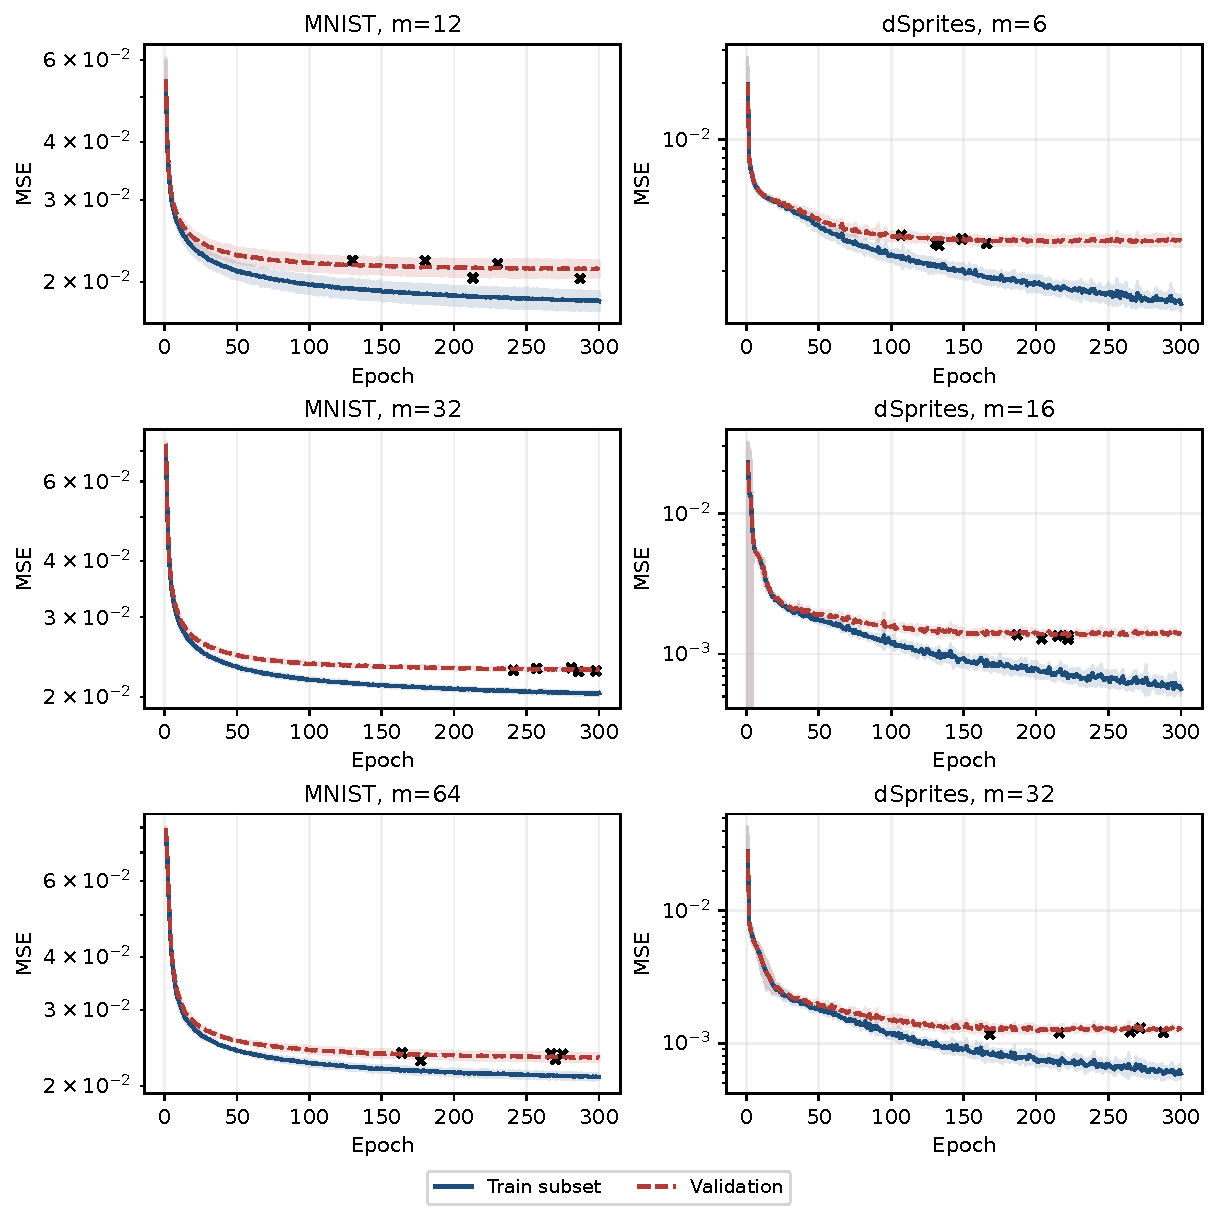
\includegraphics[width=\textwidth]{results/figures/MAKE50/learning.pdf}
\caption{Train and validation MSE, means with $\pm$1 SD bands over five
seeds. MNIST uses Gaussian and dSprites Bernoulli likelihood; $\beta=1$.
Black crosses mark each run's checkpoint selected by the validation
ELBO proxy. These diagnostic runs have no early stopping.}
\label{fig:learning}
\end{figure}

@@table:selection@@

Table~\ref{tab:selection} provides the previously omitted grid choices
based on MSE, the ELBO proxy and a linear probe. Different objectives can
select different widths and reconstruction errors. Test probe accuracy
is an auxiliary supervised outcome; it does not measure unsupervised
reconstruction quality. This comparison retains the same splits and
cached candidates, with labelled validation selection explicitly stated.

\subsection{Activity Readout: Trajectories, Thresholds and Prediction}\label{sec:au}
Figure~\ref{fig:readouts} and Table~\ref{tab:readouts} compare the two
counts on identical checkpoints. At MNIST width 64, epoch-five variable
types give $9.8\pm3.8$ and AU gives $49.4\pm8.1$; at epoch 300 both
give $6.4\pm0.5$. This example distinguishes mean agreement from
between-seed variability. The table also reports within-run changes from
50 to 300 epochs. Their magnitude depends on the condition, so no
general stability superiority is inferred from the final agreement.

@@table:readouts@@

\begin{figure}[!htbp]
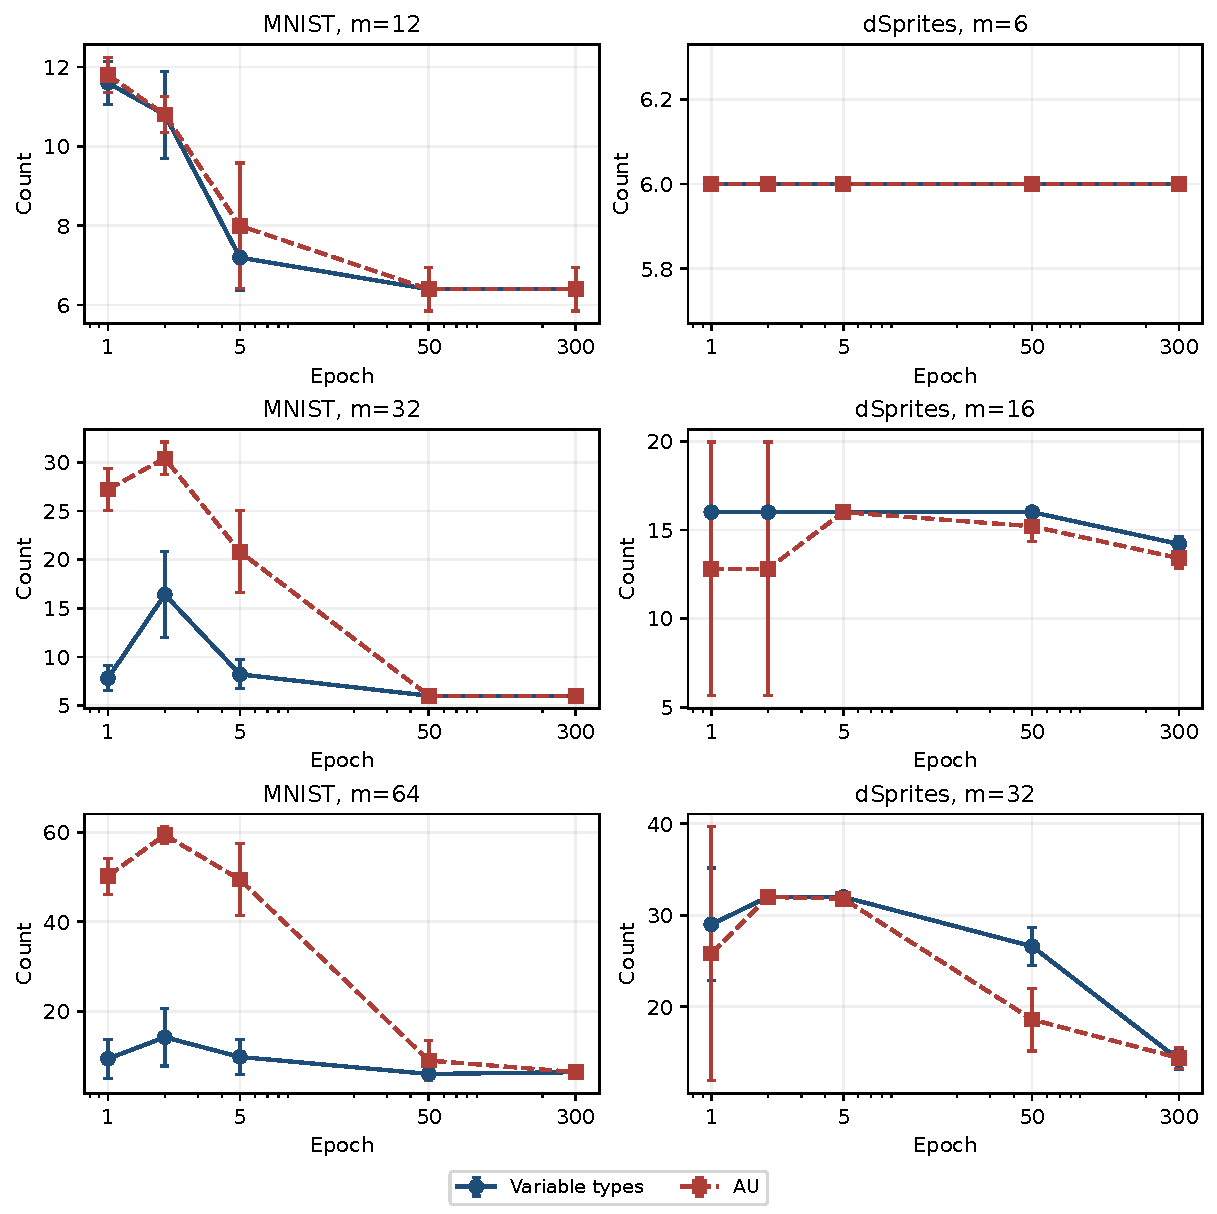
\includegraphics[width=\textwidth]{results/figures/MAKE50/readouts.pdf}
\caption{Variable-type count (active plus mixed) and AU from the same
checkpoints at epochs 1, 2, 5, 50 and 300; means and seed SDs, with lines
connecting the observed checkpoints only. $\beta=1$, Gaussian MNIST and
Bernoulli dSprites. Constant full-capacity counts are not evidence of
diagnostic stability.}
\label{fig:readouts}
\end{figure}

The threshold-only comparison in Figure~\ref{fig:delta} uses fixed
$\beta=1$ checkpoints. On CIFAR-10, $\delta=0.001$ counts every
coordinate at every tested grid width, whereas $\delta=0.1$ counts
far fewer at large widths. The inference ``no unused coordinates''
therefore depends on this threshold. Normalising the threshold changes
the diagnostic definition; it does not establish a dimension estimate.

\begin{figure}[!htbp]
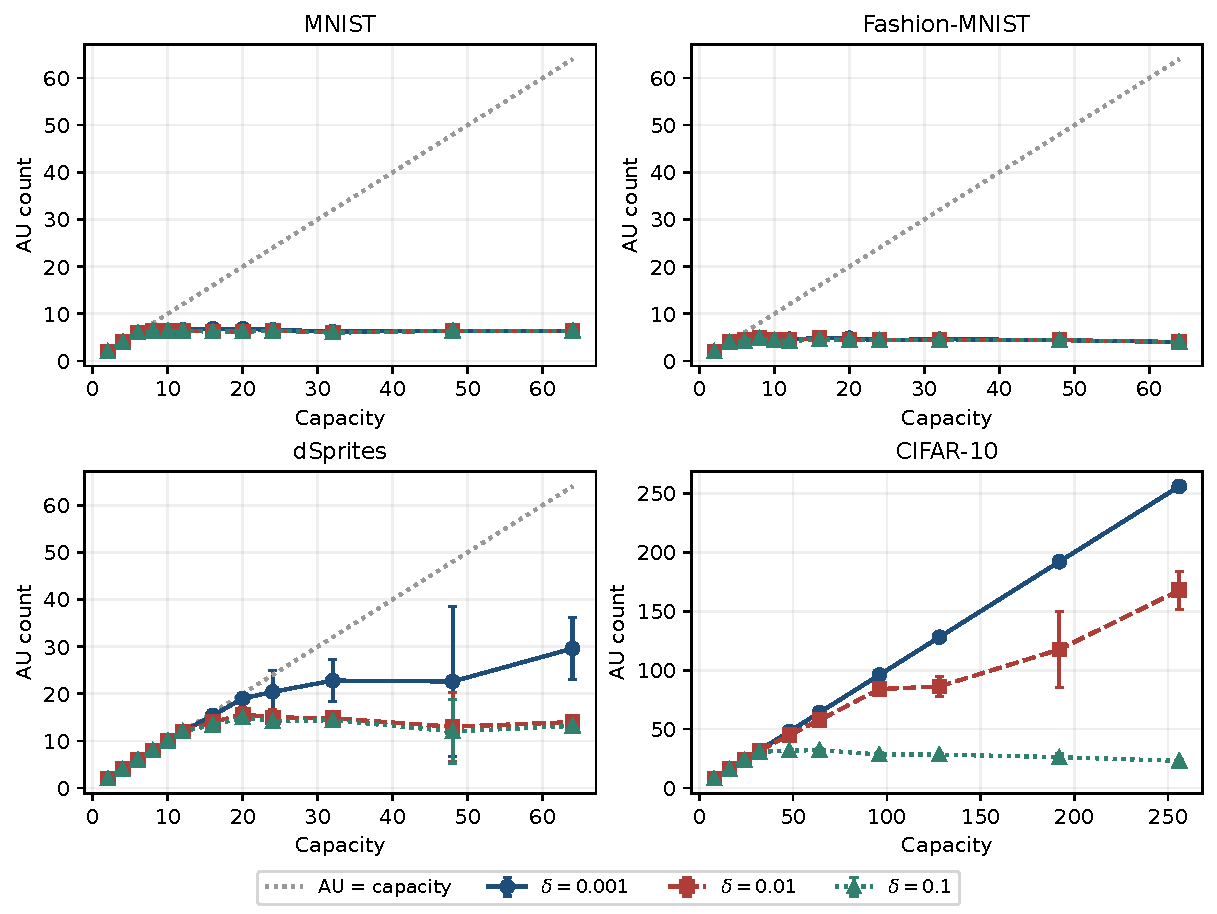
\includegraphics[width=\textwidth]{results/figures/MAKE50/delta.pdf}
\caption{AU under three thresholds on the same $\beta=1$ candidates;
mean $\pm$ seed SD. Gaussian likelihood except Bernoulli dSprites.
The diagonal is capacity. This is a readout-threshold intervention,
unlike the training/context intervention in Figure~\ref{fig:beta}.}
\label{fig:delta}
\end{figure}

The predictive task asks whether the next smaller grid candidate meets
the same seed's quality target. Each row is one validation-selected
checkpoint at a nonminimal grid width. Baseline features are validation
MSE, KL, the ELBO proxy, width, width/input-ID ratio, and the slope of
validation MSE over the last 20 recorded epochs. The three added AU
features are AU, AU/width and AU/input-ID. Standardisation is fitted
only on development rows. An $L_2$ logistic predictor is fitted on
MNIST (55 rows), with $C=@@AU_C@@$ chosen on a three-seed/two-seed
development split. Evaluation uses dSprites (55 rows), Fashion-MNIST
(55) and CIFAR-10 (45), each with five seeds. The configured
MNIST-CNN predictive condition was not executed.

The development split uses seeds 42, 123 and 777 for the inner fit and
2024 and 31337 for selecting $C$, then refits on all five. Predictors use
up to 5000 iterations. Each evaluation dataset--seed block is scored
over its complete set of nonminimal grid widths; checkpoint rows are
not resampled as independent observations.

The original internally specified analysis reported an AU-minus-baseline
AUROC improvement of $+0.108$, with a 2000-replicate seed-record bootstrap
95\% interval $[+0.059,+0.157]$. A subsequently added control used
three independent standard-normal features and one noise realisation
(generator seed 7); its separately reported improvement was $+0.098$
with interval $[-0.025,+0.227]$. Overlap of these intervals does not test
their difference or establish equivalence. These archived values are
retained as the original analysis, not as a validated positive finding:
its AUROC calculation used probabilities that can saturate numerically
under the shift between datasets.

@@table:au@@

For this revision we reconstruct both predictors at explicitly fixed
$\beta=1$, restrict rows to the declared grid, and compute AUROC from
logistic decision scores. The original cache-reading routine did not
filter $\beta$ or restrict the grid, so rerunning it after cache expansion
would also be ambiguous. Decision scores preserve ranks that are lost
when sigmoid probabilities round to exactly one. Saturation counts
appear in Appendix~\ref{app:sensitivity}. This is a corrected retrospective
analysis, not an exact replay of archived probabilities. The
AU-minus-baseline difference is now $@@AU_BASE_DIFF@@$, with interval
$[@@AU_BASE_LO@@,@@AU_BASE_HI@@]$. We also compare AU and random
predictors on the same dataset--seed blocks.
The paired mean difference is $@@AU_DIFF@@$, with a retrospective
hierarchical-bootstrap 95\% interval $[@@AU_LO@@,@@AU_HI@@]$ (2000
replicates). Each replicate resamples the three evaluation datasets and
then the five seed blocks within each selected dataset; all capacities
and both predictors remain paired within a block. Models are held fixed,
so this interval does not cover development-model fitting uncertainty.
Only three evaluation datasets are available, limiting precision of
across-condition inference. A secondary analysis averages the comparator
over 100 noise realisations (seeds 0--99), giving a paired difference
$@@AU100_DIFF@@$ and interval $[@@AU100_LO@@,@@AU100_HI@@]$ under the
same resampling. Neither analysis establishes an AU-specific benefit in
these evaluation conditions. We do not claim that AU has no information,
that the predictors are equivalent, or that lack of significance proves
insufficient power.

\subsection{Implementation Audit and Degenerate Outputs}
Two scale inconsistencies were identified in local implementations.
First, the earlier VAE loss averaged KL over latent dimensions while
summing reconstruction over input dimensions. Algebraically this gives
$\beta_{\rm effective}=\beta_{\rm nominal}/m$. The image results in
this paper come from the corrected sum-over-latents convention. The
algebra does not imply that complete optimisation trajectories or AU
counts are reproduced simply by relabelling $\beta$; the earlier
``within 1.7 units'' claim is not used here.

Second, an intermediate GECO adaptation combined per-pixel-mean
constraint values with other terms on incompatible scales. The corrected
implementation uses summed squared error and multiplies the per-pixel
target by the input dimension. Either sum or mean conventions can be
valid if the objective, target and multiplier scales are consistent.
The observed behaviour of this hard-concrete adaptation is not attributed
to the original ARM implementation.

FONDUE-VAR's active-only setting returning zero is a separate phenomenon,
not a third sum/mean defect. At MNIST's one-epoch setting it returns zero
on all five trials; no final VAE exists for these outputs.
Table~\ref{tab:var} shows both settings and their quality/validity counts.

@@table:var@@

\section{Discussion}\label{sec:discussion}
The most direct evidence is the paired MNIST comparison: under the tested
model family, grid and target, the implemented ID-guided selector gives
no recorded-training-cost advantage over ascending search. Its reliability
checks reject the other three datasets, but those repeated rejections
share a reference bank. They indicate failure of this applicability check
under these representations, not that ID methods generally cannot work
on those datasets. Different reference architectures, grids, targets or
reliable estimators could change the comparison.

Regularisation ranges and AU-threshold responses are different
measurements. Some large dimension ranges reflect fallback, grid scale
or a changing quality target. A constant output can be fixed by design
or by an unvaried implementation argument. Thus the evidence supports
method- and dataset-dependent responses, not a universal robustness
ranking. The archived positive AU-versus-baseline result is not robust
to preserving logistic-score rankings instead of rounded probabilities.
The corrected predictive comparison does not establish an AU-specific
advantage over the matched random-feature controls.

Several limits remain material. The pruning rows evaluate dimension
transfer through local adaptations, including nearest-grid rounding;
their native model performance and exact-source implementations are not
compared. Complete ID/evaluation timings are missing, so a strict
end-to-end cost ranking cannot be reconstructed. The ID selector's
expansion branch is ineffective. A fixed-quality $\beta$ intervention,
a correctly varied ARD selection weight with source-matched relevance
scoring, and an exact ARM comparison require new training and are not
claimed as completed experiments. The single split and shared references
also limit uncertainty estimates. These restrictions are preferable to
interpreting the current records as broader evidence than they provide.

The synthetic experiments in Appendix~\ref{app:synthetic} illustrate
scale dependence and the effect of zeroing low-variance coordinates.
Their counts are observations under a particular loss and coordinate
system. They do not show that topology predicts the number of active
axes, and their preprocessing prevents treating them as clean estimates
of held-out generalisation.

\section{Conclusions}\label{sec:conclusion}
We compared latent-width selection rules using common candidate-model
families, explicit validation targets and a documented training-time
account. At the primary MNIST setting, ID guidance and ascending search
select the same six-dimensional VAE, while ID guidance incurs more
recorded training time. ID estimates depend on representation and sample
size; AU counts depend on their readout threshold. The paired predictive
comparison does not establish an AU-specific advantage over the evaluated
random-feature controls. Dimension variation across regularisation
contexts differs by method and dataset, without a transferable ranking.
These findings delimit what ID and AU alone can establish about the
capacity needed for a chosen reconstruction quality under the tested
conditions.

\authorcontributions{Conceptualization, C.O., M.D. and K.J.; methodology,
C.O. and K.J.; software, C.O. and M.D.; validation, C.O., M.D. and K.J.;
formal analysis, C.O. and K.J.; investigation, C.O., M.D. and K.J.;
writing---original draft preparation, C.O. and K.J.; writing---review and
editing, C.O., M.D. and K.J.; supervision and project administration, K.J.}
\funding{This research was funded by JSPS KAKENHI Grant Numbers
JP24K15115 and JP26K14984, by the Tokyo City University Priority Research
[Intelligent Technology Optimization Research Unit: ORBIT], by a
Cooperative Research Project of the Research Institute of Electrical
Communication (RIEC), Tohoku University, and by a Research Grant from the
Telecommunications Advancement Foundation (TAF).}
\institutionalreview{Not applicable.}
\informedconsent{Not applicable.}
\dataavailability{The image datasets are publicly available from their
cited sources. Source records, reaggregation code and the resulting
machine-readable tables are identified in Appendix~\ref{app:inventory}.
No public archive DOI is assigned in this manuscript.}
\acknowledgments{Generative-AI assistance was used for experimental-code
drafting and refactoring and English-language editing in the earlier
manuscript preparation. OpenAI Codex assisted with the present record
audit, reaggregation, figure preparation and manuscript revision.
Responsibility for the scientific content rests with the authors.}
\conflictsofinterest{The authors declare no conflicts of interest.}

\appendixtitles{yes}
\appendixstart
\appendix
\section{Quality Targets and Outcome Accounting}\label{app:targets}
@@table:anchors@@

\subsection{Independent Outcome Counts}\label{app:outcomes}
The following tables separate the original combined state from flags and
final-model quality. A budget flag can coexist with ID fallback. The
pruning wrapper did not enforce the ordinary selector budget during
training, so its zero budget-flag count is not evidence of equal budget
control. All valid returned models, including those from budget-exceeded
trials, contribute to the primary means. Degenerate outputs contribute
to raw-count and cost summaries but not to MSE.
@@table:outcomes0@@
@@table:outcomes1@@

\section{Coverage and Implementation Details}\label{app:coverage}
\begin{table}[H]
\caption{Executed coverage. Each image method row has five training
seeds at each listed context. Additional diagnostic experiments have
their own seed units.}
\label{tab:coverage}\small
\begin{tabularx}{\textwidth}{lXX}\toprule
Experiment & Dataset coverage & Contexts / counts \\\midrule
Fourteen ordinary selectors/controls & All four image datasets & Five $\beta$ values; $14\times4\times5\times5=1400$ method records \\
GECO adaptation & All four & Five anchor-derived constraints; 100 records \\
ARD adaptation & All four & Fixed selection-stage weight one; five repeated contexts, 100 records \\
ID-reference bank & All four & Three widths $\times$ three seeds each, shared across contexts \\
Train/validation and readout trajectories & MNIST: 12, 32, 64; dSprites: 6, 16, 32 & $\beta=1$, five seeds each; 30 runs \\
AU prediction & Develop: MNIST; evaluate: dSprites, Fashion-MNIST, CIFAR-10 & $\beta=1$; 55 development and 155 evaluation rows \\
Synthetic diagnostic & Swiss roll and torus & Six capacities, three seeds, two scaling options; 72 runs \\
\bottomrule\end{tabularx}
\end{table}

The fourteen ordinary method records comprise MSE/ELBO-proxy/probe grid
selection, coarse search, fixed width, FONDUE, two FONDUE-VAR settings,
ID guidance with and without AU recording, ascending+$Q$, and coarse,
FONDUE and FONDUE-VAR with added $Q$. Removing AU recording does not
change the ID selection decisions; its overhead was not separately
timed. Machine-readable results include all fourteen, even when only
the principal comparisons are printed.

@@table:splits@@
The split index arrays are reconstructed from the loader specification,
not recovered as an independently archived execution-time split file.
The MNIST and Fashion-MNIST tokens agree because their official pool
sizes and index rules agree; their images are different. A compressed
copy is supplied as \path{results/make50/reconstructed_split_indices.npz}.
TwoNN uses Euclidean nearest-neighbour distances, excludes zero first
distances and the empirical-CDF endpoint, and fits the log survival
curve against the log distance ratio through the origin. The MLE
cross-check averages local reciprocal mean-log-distance-ratio estimates
over valid points at $k=10$. Both estimates are floored at one in the
local implementation.

@@table:epochs@@

\subsection{Pruning and Relevance Adaptations}\label{app:adaptations}
The GECO adaptation uses Adam at $10^{-3}$, batches of 128 in stored
order, 300 epochs and hard-concrete parameters $\gamma=-0.1$,
$\zeta=1.1$ and temperature $2/3$. Initial gate log-odds are 2. The
constraint is summed squared reconstruction error minus
$D_{\rm input}T_{D,s}$, with moving-average coefficient 0.99. A squared
softplus multiplier is clamped to $[10^{-6},10^6]$ and updated by ascent
on that moving-average violation. KL is gate-masked; the expected gate
penalty is enabled only when the moving-average constraint is satisfied.
The final readout counts deterministic gates above 0.5. Its training
constraint uses squared error even on dSprites; the transferred ordinary
VAE there uses Bernoulli reconstruction. Consequently the candidate
likelihood convention does not imply identical pruning-stage objectives.

@@table:pruning@@

The ARD adaptation reserves the first 10\% (1800 examples) of its
training array for prior estimation and trains on the remainder.
It updates $p_j=\operatorname{mean}(\mu_j^2+\sigma_j^2)$ every ten
epochs and after training, clipping to $[10^{-6},10^6]$.
This uses analytic posterior second moments in a fixed subset, rather
than a periodically resampled encoded-data pool. Selection training uses
reconstruction plus Gaussian KL at unit weight. On the first 512
training examples it computes
\begin{equation}
 w_j=\operatorname{mean}_{x,k}
 [g_k(\mu(x)+\sqrt{p_j}e_j)-g_k(\mu(x))]^2,
 \qquad q_j=w_jp_j,
 \label{eq:ardlocal}
\end{equation}
and keeps the smallest number of descending scores reaching 99\% of
their total. The finite difference is not divided by its squared step.
Locally it already contains a factor $p_j$, so multiplication by $p_j$
again differs from a Jacobian-squared times variance score. The stored
counts are therefore labelled an \emph{ARD adaptation}; this difference
cannot be removed by correcting the prose. The Gaussian approximation
alone is not an original-source deviation. Identical relevance arrays
and counts across contexts are checked in the numerical audit; they
represent repeated fixed settings, not a $\beta$ sweep.

The FONDUE description-based classifier was checked against the public
repository \url{https://github.com/bonheml/VAE_learning_dynamics} at
commit \texttt{f6d6e66b536bcbe635392d3438338949d4dc8730}. The local
implementation uses the stated posterior-variance categories with one
exponentiation and TwoNN; equivalence to the public execution path and
the original experiment configuration is not asserted. As a historical
reference, the source reports dSprites selection $12.2\pm0.4$ at one
epoch~\cite{bonheme2022fondue}, versus $4.2\pm0.4$ here at $\beta=1$.
This unmatched-setting difference is not proof of an implementation
error, nor a reproduction of the original benchmark.

\subsection{Threshold-Only and Quality-Margin Analyses}\label{app:sensitivity}
The retrospective predictive analysis uses Python @@PYTHON@@,
NumPy @@NUMPY@@ and scikit-learn @@SKLEARN@@. Table~\ref{tab:saturation}
documents probability saturation in this reconstruction. The original
predictor's complete environment and row-level probabilities were not
saved, so its exact floating-point results cannot be verified from the
summary alone. Row-level decision scores and probabilities for the
current reconstruction are saved in \path{results/make50/au_predictions.csv}.
@@table:saturation@@

The main AU-threshold figure uses identical checkpoints for all three
$\delta$ values. Across the full ladder, the fractions of CIFAR-10
grid/seed candidates with AU equal to capacity are given below.
These counts use ten widths and five seeds per $\beta$; their rows are
not 50 independent datasets.
@@table:delta_rates@@

For a separate retrospective quality-margin check, the complete cached
grid at $\beta=1$ is held fixed and the smallest satisfying width is read
out for each margin, without retraining or changing the anchor.
Table~\ref{tab:margin} reports this full-grid criterion, not the path or
cost of any restricted-window selector. No FONDUE-threshold or ARD-99\%
sensitivity training was executed, so no response of those rules to their
own readout thresholds is claimed.
@@table:margin@@

\section{Synthetic Scale and Ablation Diagnostic}\label{app:synthetic}
Swiss-roll points are $(t\cos t,h,t\sin t)$ with
$t\sim U[1.5\pi,4.5\pi]$ and $h\sim U[0,1]$. Torus points are
$((3+\cos\phi)\cos\theta,(3+\cos\phi)\sin\theta,\sin\phi)$ with
independent angles uniform on $[0,2\pi]$. Each has 5000 examples,
generation seed zero, and independent Gaussian coordinate noise with
SD 0.01. The first 4500 are used for fitting and the remaining 500 for
the reported diagnostic. Per-coordinate standardisation in the stored
experiment was fitted to all 5000 before splitting. This is disclosed
as preprocessing leakage; the results are descriptive, not clean
held-out test estimates.

The FC VAE uses widths 128 and 64, reversed in its decoder, ReLU hidden
activations, a linear output, Adam at $10^{-3}$, batch 128, 300 epochs,
$\beta=1$ and seeds 42, 123 and 777. At the last checkpoint, coordinates
with posterior-mean variance at most 0.01 on the 500 diagnostic examples
are zeroed and MSE is recomputed on those same examples.
Table~\ref{tab:synthetic} reports the standardized runs. There is no
separate test set in this stored experiment.

@@table:synthetic@@

Both noise-free generating surfaces have intrinsic dimension two and
are represented here in three ambient coordinates. A Swiss-roll patch
does not thereby have minimum embedding dimension three. Observing
three active coordinates under this loss is not a topological theorem.
The earlier manuscript said its synthetic coordinates were standardized;
the implementation audit found a mismatch between that description and
the executed preprocessing. On the unstandardized Swiss roll the height
coordinate has much smaller variance than the other coordinates, making
its omission inexpensive in squared error. This scale observation does
not alone prove the complete causal explanation of every earlier AU
result.

\section{Reproducibility Inventory and Remaining Records}\label{app:inventory}
The reaggregation entry point is
\path{src/make50/rebuild_review.py}; it reads saved JSON and configuration
files and writes numerical tables, six figures and the paired predictive
analysis without VAE retraining. The manuscript assembly entry point is
\path{src/make50/build_manuscript.py}. The generated main TeX embeds its
table contents and references the figure PDFs. Compile from the project
root with \texttt{pdflatex} repeatedly until references settle.

\begin{table}[H]
\caption{Source-to-output map for the present revision. Paths below are
relative to the project root.}
\label{tab:inventory}\footnotesize
\begin{tabularx}{\textwidth}{lX}\toprule
Evidence & File or directory \\\midrule
Configuration & \path{config/experiment_config_MAKE49.json} \\
Ordinary method records & \path{results/make49/stage4_methods.json} \\
Pruning records & \path{results/make49/stage7_b7b8.json} \\
Candidate metrics and latent variances & \path{results/make49/stage4_cache/} \\
Train/validation and readout trajectories & \path{results/make49/stage3_e7a_e2.json} \\
ID representation diagnostics & \path{results/make49/stage5_e3_reference.json} \\
Original AU prediction result & \path{results/make49/stage5_e4_au_value.json} \\
Synthetic runs & \path{results/make49/stage6_e6_synthetic.json} \\
All audited method rows & \path{results/make50/method_results.csv} \\
Paired AU analysis & \path{results/make50/au_paired.json} \\
Snapshot identities & \path{results/make50/source_manifest.json} \\
Figures & \path{results/figures/MAKE50/} \\
\bottomrule\end{tabularx}
\end{table}

Method-level row identifiers are
(dataset, method, candidate seed, $\beta$ or context). Candidate keys
also contain width, requested epochs and stopping option. Every
configuration/dataset--method--context cell in the main method archive
has five seeds; this is checked during reaggregation. The ARD repetition
does not create five distinct selection-weight conditions. Individual
early off-grid cache entries are not all retained, although their final
metrics and training traces remain in the method records. The original
test predictions, full model checkpoints and independent ID/evaluation
timings are not reconstructed from missing files.

The local change record documents the initial specification on
12 September; the switch to Bernoulli dSprites after collapse diagnostics;
the move of ID estimation from an impossible 10,000-example validation
sample to training data; trajectory runs without early stopping; and
the 13 September reference-width, run-accounting and degenerate-output
clarifications. The random-feature control was added after the primary
predictive analysis. In this revision, anchor-cost completion, paired AU
inference, quality-margin rereading and explicit implementation auditing
are retrospective. None is relabelled as a publicly preregistered test.
